\iffalse
\let\negmedspace\undefined
\let\negthickspace\undefined
\documentclass[journal,12pt,twocolumn]{IEEEtran}
\usepackage{cite}
\usepackage{amsmath,amssymb,amsfonts,amsthm}
\usepackage{algorithmic}
\usepackage{graphicx}
\usepackage{textcomp}
\usepackage{xcolor}
\usepackage{txfonts}
\usepackage{listings}
\usepackage{enumitem}
\usepackage{mathtools}
\usepackage{gensymb}
\usepackage[breaklinks=true]{hyperref}
\usepackage{tkz-euclide} 
\usepackage{listings}
\usepackage{gvv}
%
%\usepackage{setspace}
%\usepackage{gensymb}
%\doublespacing
%\singlespacing

%\usepackage{graphicx}
%\usepackage{amssymb}
%\usepackage{relsize}
%\usepackage[cmex10]{amsmath}
%\usepackage{amsthm}
%\interdisplaylinepenalty=2500
%\savesymbol{iint}
%\usepackage{txfonts}
%\restoresymbol{TXF}{iint}
%\usepackage{wasysym}
%\usepackage{amsthm}
%\usepackage{iithtlc}
%\usepackage{mathrsfs}
%\usepackage{txfonts}
%\usepackage{stfloats}
%\usepackage{bm}
%\usepackage{cite}
%\usepackage{cases}
%\usepackage{subfig}
%\usepackage{xtab}
%\usepackage{longtable}
%\usepackage{multirow}
%\usepackage{algorithm}
%\usepackage{algpseudocode}
%\usepackage{enumitem}
%\usepackage{mathtools}
%\usepackage{tikz}
%\usepackage{circuitikz}
%\usepackage{verbatim}
%\usepackage{tfrupee}
%\usepackage{stmaryrd}
%\usetkzobj{all}
%    \usepackage{color}                                            %%
%    \usepackage{array}                                            %%
%    \usepackage{longtable}                                        %%
%    \usepackage{calc}                                             %%
%    \usepackage{multirow}                                         %%
%    \usepackage{hhline}                                           %%
%    \usepackage{ifthen}                                           %%
  %optionally (for landscape tables embedded in another document): %%
%    \usepackage{lscape}     
%\usepackage{multicol}
%\usepackage{chngcntr}
%\usepackage{enumerate}

%\usepackage{wasysym}
%\documentclass[conference]{IEEEtran}
%\IEEEoverridecommandlockouts
% The preceding line is only needed to identify funding in the first footnote. If that is unneeded, please comment it out.

\newtheorem{theorem}{Theorem}[section]
\newtheorem{problem}{Problem}
\newtheorem{proposition}{Proposition}[section]
\newtheorem{lemma}{Lemma}[section]
\newtheorem{corollary}[theorem]{Corollary}
\newtheorem{example}{Example}[section]
\newtheorem{definition}[problem]{Definition}

\newcommand{\BEQA}{\begin{eqnarray}}
\newcommand{\EEQA}{\end{eqnarray}}
\newcommand{\define}{\stackrel{\triangle}{=}}
\theoremstyle{remark}
\newtheorem{rem}{Remark}


\begin{document}


\bibliographystyle{IEEEtran}


\vspace{3cm}

\title{
	Question 1.5.9
}

\author{
	EE22BTECH11054 - Umair Parwez
}	

\maketitle
\newpage


\renewcommand{\thefigure}{\theenumi}
\renewcommand{\thetable}{\theenumi}


\textbf{Question 1.5.9:}

Given triangle $ABC$ with vertices, 
\begin{align}
	\vec{A} = \myvec{1\\ -1}, \vec{B} = \myvec{-4\\ 6}, \vec{C} = \myvec{-3\\ -5}
\end{align}
Find the points of contact, $\vec{E}_3$ and $\vec{F}_3$, of the incircle with sides $AC$ and $AB$ respectively.
\fi
\textbf{Solution:}

Required to find points of contact, $\vec{E}_3$ and $\vec{F}_3$, of incircle with sides $AC$ and $AB$ respectively.
From previous questions we know the coordinates of the incircle are : 
\begin{align}
	\vec{I} &= 
	\myvec {
		\frac{-53-11\sqrt{37}+7\sqrt{61}+\sqrt{2257}}{12} \\ 
		\frac{5-\sqrt{37}+5\sqrt{61}-\sqrt{2257}}{12}
	} \\
	&= \myvec{-1.47756 \\ -0.79495}
\end{align}
Radius of incircle is :
    \begin{align}
		r &= \frac{185+41\sqrt{37}-37\sqrt{61}-\sqrt{2257}}{6\sqrt{74}} \\
		&= 1.89689
	\end{align}
Equation of incircle is : 
\begin{align}
	{\norm{ \vec{x}-\vec{I} }}^2 = {r}^2 \label{eq:circle}
\end{align}
points $\vec{A}$, $\vec{B}$ and $\vec{C}$ are : 
\begin{align}
	\vec{A} = \myvec{
		1\\
		-1
	}, 
	\vec{B} = \myvec{
		-4\\
		6
	}, 
	\vec{C} = \myvec{
		-3\\
		-5
	}
\end{align}
Parametric equation of any line is of the form :
\begin{align}
	\vec{x} = \vec{A} + k\vec{m} \label{eq:param}
\end{align}
We can substitute \eqref{eq:param} in \eqref{eq:circle}, and we get : 
\begin{align}
	{\norm{ \vec{A}+k\vec{m}-\vec{I} }}^2 &= {r}^2 \\
	\implies (k\vec{m} + (\vec{A} - \vec{I}))(k\vec{m} + (\vec{A} - \vec{I})) &= {r}^2 \\
	\implies k^2 \norm{\vec{m}}^2 + 2k\vec{m}^{\top} (\vec{A}-\vec{I}) + \norm{\vec{A}-\vec{I}}^2 &= {r}^2 
\end{align}
The discriminant of the above quadratic is,
\begin{align}
	\Delta = 4(\vec{m}^{\top}(\vec{A}-\vec{I}))^2 - 4\norm{\vec{m}}^2(\norm{\vec{A}-\vec{I}}^2 - r^2) \label{eq:Delta}
\end{align} 
If,
\begin{align}
	\Delta = 0
\end{align}
Then the line given by \eqref{eq:param} is tangent to the incircle and the value of $k$ will be given by :
\begin{align}
	k = -\frac{\vec{m}^{\top}(\vec{A} - \vec{I})}{\norm{\vec{m}}^2} \label{eq:k}
\end{align}
Upon substituting $k$ back into \eqref{eq:param}, we will obtain the point of contact of the line with the incircle.
\begin{enumerate}
	\item Finding $\vec{E}_3$ :\\
		Parametric equation of $AC$ is,
		\begin{align}
			\vec{x} = \vec{A} + k\vec{m} \label{eq:AC}
		\end{align}
		where,
		\begin{align}
			\vec{m} = \vec{A} - \vec{C}
		\end{align}	
		First we confirm value of $\Delta$ for $AC$,
		\begin{align}
			\Delta &= 4(\vec{m}^{\top}(\vec{A}-\vec{I}))^2 - 4\norm{\vec{m}}^2(\norm{\vec{A}-\vec{I}}^2 - r^2)\\	
			&= 4(9.09004)^2 - 4(32)(6.18035-3.59819) \\
			&= 0
		\end{align}
		Therefore, $AC$ is tangent to the incircle, and value of $k$ is given by, 
		\begin{align}
			k &= -\frac{\vec{m}^{\top}(\vec{A} - \vec{I})}{\norm{\vec{m}}^2} \\
			&= -\frac{(\vec{A}-\vec{C})^{\top}(\vec{A} - \vec{I})}{\norm{\vec{A}-\vec{C}}^2}
		\end{align}
		Substituting the values, we get,
		\begin{align}
			k = \frac{-4-\sqrt{37}+\sqrt{61}}{2} \label{k:AC} 
		\end{align}
		Substituting \eqref{k:AC} into \eqref{eq:AC}, we get the value of $\vec{E}_3$,
		\begin{align}
			\vec{E}_3 = \myvec{
				\frac{-2-\sqrt{37}+\sqrt{61}}{2}\\ 
				\frac{-6-\sqrt{37}+\sqrt{61}}{2}
			}
		\end{align}
	\item Finding $\vec{F}_3$ :\\
		Parametric equation of $AB$ is,
		\begin{align}
			\vec{x} = \vec{A} + k\vec{m} \label{eq:AB}
		\end{align}
		where,
		\begin{align}
			\vec{m} = \vec{A} - \vec{B}
		\end{align}	
		First we confirm value of $\Delta$ for $AB$,
		\begin{align}
			\Delta &= 4(\vec{m}^{\top}(\vec{A}-\vec{I}))^2 - 4\norm{\vec{m}}^2(\norm{\vec{A}-\vec{I}}^2 - r^2)\\	
			&= 4(13.82315)^2 - 4(74)(6.18035-3.59819) \\
			&= 0
		\end{align}
		Therefore, $AB$ is tangent to the incircle, and value of $k$ is given by, 
		\begin{align}
			k &= -\frac{\vec{m}^{\top}(\vec{A} - \vec{I})}{\norm{\vec{m}}^2} \\
			&= -\frac{(\vec{A}-\vec{B})^{\top}(\vec{A} - \vec{I})}{\norm{\vec{A}-\vec{B}}^2}
		\end{align}
		Substituting the values, we get,
		\begin{align}
			k = \frac{-37-4\sqrt{37}+\sqrt{2257}}{74} \label{k:AB} 
		\end{align}
		Substituting \eqref{k:AB} into \eqref{eq:AB}, we get the value of $\vec{F}_3$,
		\begin{align}
			\vec{F}_3 = \myvec{
				\frac{-111-20\sqrt{37}+5\sqrt{2257}}{74}\\ 
				\frac{185+28\sqrt{37}-7\sqrt{2257}}{74}
			}
		\end{align}
\end{enumerate}
Diagram is shown below,
\begin{figure}[h]
	\centering
	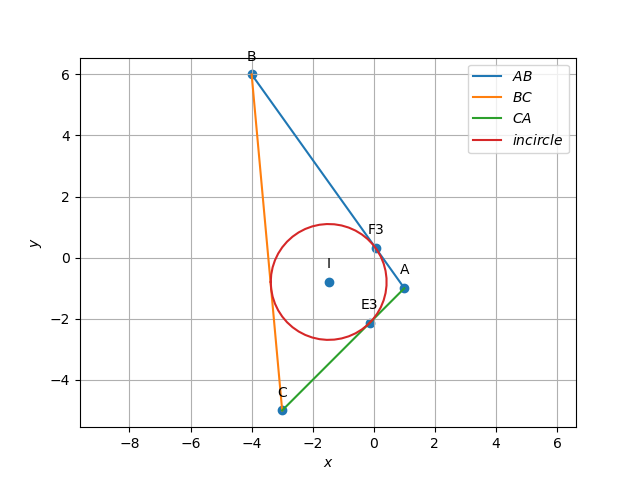
\includegraphics[width=\columnwidth]{./figs/Diagram.png}
	\caption{Points of contact of incircle}
	\label{fig:Incircle}
\end{figure}



